\section*{Side-Chain Entropy in Protein Design}
\label{sec:side_chain_entropy_in_protein_design}
Another approach to the question of side-chain entropy, and one that has only become feasible with recent advances, is to look at its role in the \emph{de novo} design of proteins. The prospect of explicitly calculating all of the thermodynamic parameters involved in folding a protein is already a daunting challenge. Performing these calculations while iterating through all of sequence space to find a specific protein fold is flat out impossible. For that reason, \emph{de novo} design algorithms make simplifying assumptions about what sorts of thermodynamic parameters are important in determining a protein's shape\cite{Lippow:2007p360}. Most of these algorithms will randomly iterate through sequence space, stopping at regular intervals to minimize the protein structure (for example, by simulated annealing) followed by calculation of scoring function which will determine if the structure should be kept or rejected.

RosettaDesign is just such an algorithm, and Hu and Kuhlman have used it to investigate the role of side-chain entropy in the \emph{de novo} design process\cite{Hu:2006p68}. The advantage of this approach is that it requires only a small modification to the design algorithm. The portion of the algorithm which handles iteration through sequence space and minimization of the mutated structures does not need to be modified. Instead, Hu and Kuhlman include a step which involves Monte Carlo sampling to generate an ensemble of structures used to calculate side-chain entropy and free energy. They then substitute free energy as the Metropolis acceptance criterion in place of minimized energy, which was used as the criterion in the original algorithm.

To calculate side-chain entropy, they look at the side-chains in the Monte Carlo ensemble and, for each residue, they iterate through the available rotamers, summing a probability based entropy. In equation form, this is: \[
	S = -R \sum^{nres}_{i=1}\sum^{nrot}_{r=1}p(r,i)ln[p(r,i)]
\] where $nres$ is the number of residues in the protein and $nrot$ is the number of rotamers for the residue. What's notable about this method of calculating entropy is that it explicitly neglects pair-wise terms. The entropy for each residue is calculated independently of the other residues in the chain. This significantly simplifies the task of determining side-chain entropy, but is it a realistic assumption?

To answer that question, they first calculated side-chain entropy in three different ways. The first was simply the enumeration, given above, that they planed to use in the design algorithm. The second method involved treating clusters of 6 neighboring side-chains as a unit and enumerating over the various combinations of rotamers for each cluster. The final method involved treating each dihedral angle in each side-chain independently. Comparing these three techniques, they find that the difference between an independent treatment of the side-chains and treating clusters of side-chains is on the order of $10^{-2} kcal/mol$, which the authors judge to be insignificant. Treating each dihedral angle independently yields a more significant overestimation of the side-chain entropy, indicating that there is covariant motion within a side-chain but not between side-chains.

With these results in hand, they proceeded to carry out repacking simulations (essentially, the design algorithm without mutating any residues) using both the original scoring metric and the modified metric including side-chain entropy. Dividing the residues between those which are near the surface and those buried in the protein's interior, they were able to measure a change in side-chain entropy upon burial (Figure~\ref{fig:surface_vs_buried}). As expected, they find that the longer, more flexible side chains suffer a greater entropy penalty when buried, but when accounting for the difference between the average energy of the side-chains and the energy of the most stable side-chain conformation, they find the difference is less noticeable. Only four amino acids (Met, Arg, Gln, and Glu) have a greater than $0.3 kcal/mol$ advantage when positioned near the surface.

\begin{figure}[h]
	\center
	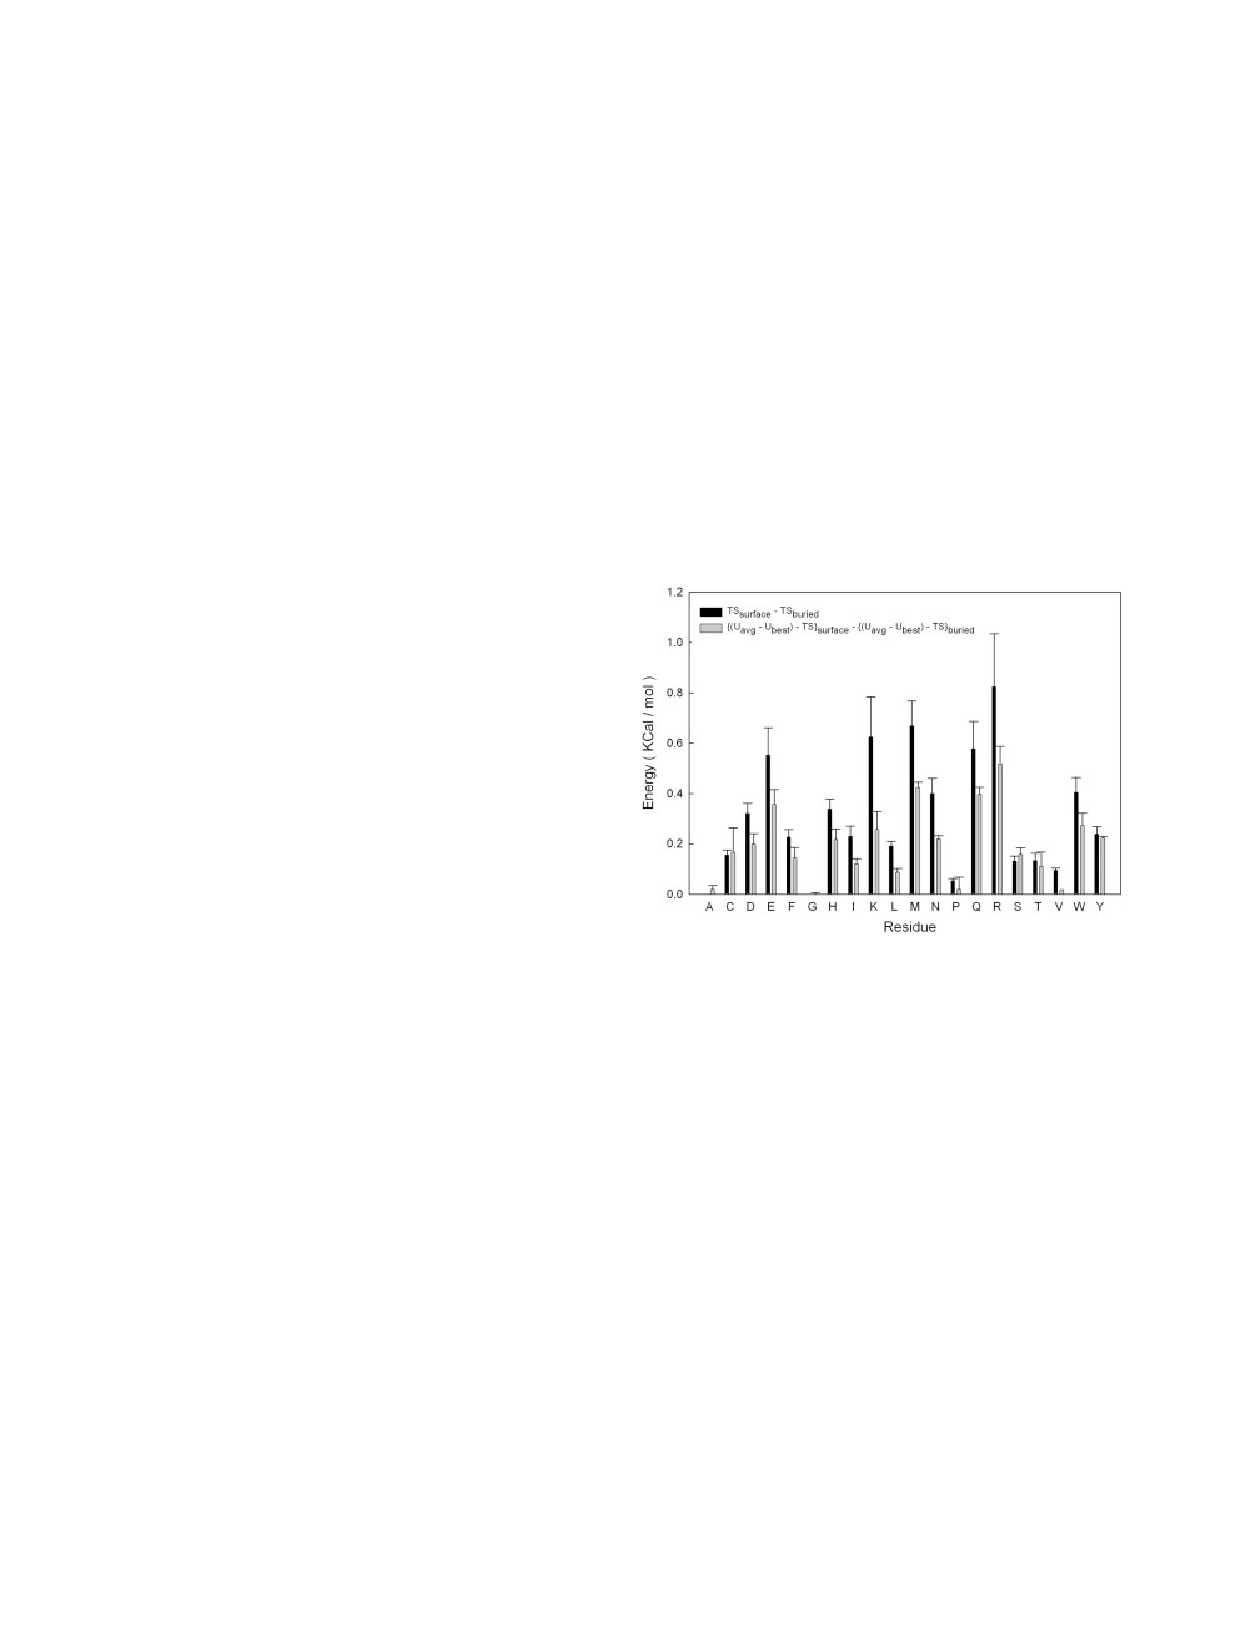
\includegraphics{surface_vs_buried}
	\caption{(Borrowed from \cite{Hu:2006p68}) Changes in side-chain conformational entropy and free energy between surface and buried positions. The black bars show the change in entropy (TS) when a residue is buried whereas the gray bars compare average free energies ($\mathrm{U_{avg}}$ - TS) obtained with the explicit side-chain entropy model to the energies that are calculated with the standard RosettaDesign model ($\mathrm{U_{best}}$). The gray bars indicate the net effect that the explicit side-chain entropy model has on the environmental preferences of the amino acids.}
	\label{fig:surface_vs_buried}
\end{figure}

From this result, the authors expected that inclusion of side-chain entropy in their design algorithm would not have a significant impact on the results. To verify this, they carried design experiments for 110 naturally occurring proteins in an attempt to recover the native sequence. Comparing the designed sequences from both the original algorithm and the modified algorithm, the success rate is not materially affected by the inclusion of side-chain entropy. In both cases, approximately one-third of the native sequence residues were selected by \emph{de novo} design. There was a noticeable change in the frequency with which the longer amino acids were buried when including side-chain entropy, but not as large an effect as when other parameters of the energy calculation, such as solvation energy, were omitted.

While these results would appear to indicate that side-chain entropy is not vital for determining protein structure, the technique used depends on the pairwise entropy interactions being ignored. Even though a proof of concept experiment seemed to indicate that this was a valid simplification, entropy is a tricky quantity to characterize. Because of the fact that it is an ensemble property, what might appear to be a small discrepancy in a small experiment, might become a large error in a full scale simulation. So, what happens if pairwise contributions are accounted for?

This is precisely the question Sciretti, \emph{et al.} attempted to answer\cite{Sciretti:2008p361}. Using a pairwise approximation applied via the Belief Propagation (BP) technique, they are able to calculate free energy and use it as a minimization criteria. Before undertaking a full protein design experiment, however, they begin by evaluating the conformational side-chain entropy for a three residue stretch in an SH3 domain. Considering all possible rotamer combinations for all possible amino acid combinations for this stretch leads to a few million calculations. This yields an exact calculation of the side-chain entropy for the stretch, which they compare to the same calculations performed using the BP technique. The results validate the use of BP for side-chain entropy calculations, as the results using BP are essentially identical.

As further validation, they allow the side-chains of the remaining residues (beside the three being mutated) to relax normally. The problem in this case is intractable for an exact calculation, but they were able to verify that the BP results from these simulations were essentially the same as those from the above case where all but the three mutated residues had their positions fixed. As a final validation of the BP method, they measure free energy as the temperature nears absolute zero and find that free energy converges with potential energy (the entropy contribution disappears at absolute zero). Armed with this evidence that BP is a powerful technique for evaluating the free energy of protein structures, they then undertook a series of \emph{de novo} design experiments.

In the first set of design runs, they carried out calculations at absolute zero using potential energy as the evaluation criteria. In the second set of runs, they carried out calculations at a temperature of $T=0.6$ (in $RT$ units), and using the BP technique, evaluated structures by free energy. They then held the structures fixed, and calculated free energy at a range of temperatures for both sets (Figure~\ref{fig:BP_vs_SA}). The structures evaluated by potential energy at absolute zero were, unsurprisingly, also the lowest in terms of free energy at absolute zero. What was unexpected was that, while the structures selected using BP at $T=0.6$ had significantly higher free energy at the low temperatures, they had significantly lower free energies at the more physiologically relevant temperature than the first set of candidates.

\begin{figure}[h]
	\center
	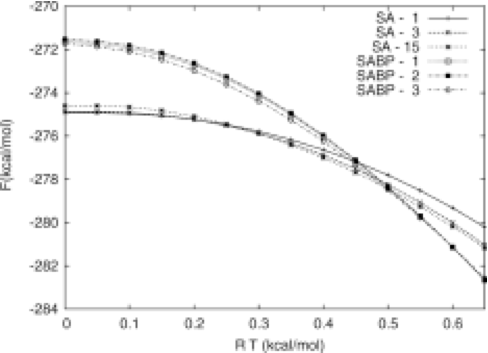
\includegraphics{BP_vs_SA}
	\caption{(Borrowed from \cite{Sciretti:2008p361}) Free energies vs temperature for some of the best ranking sequences as found by Simulated Annealing alone (SA) and Simulated Annealing with Belief Propagation (SABP). The authors have checked that BP free energies converge to SA energies at low temperature, suggesting that for these sequences the pair-wise approximation is reliable also at low temperatures.}
	\label{fig:BP_vs_SA}
\end{figure}

In fact, the authors point out that the difference between these two sets at both the high and low temperatures is great enough that there would be little chance of finding the structures in one set using the selection criteria from the other for the design phase, and then switching scoring methods when picking candidates. In other words, a \emph{de novo} protein design methodology which accounts for free energy will give very different results than one which does not. Perhaps the most surprising outcome of these experiments, however, is that the designed proteins in both sets recover only 35-55\% of the native structure, a result not entirely inconsistent with the work of Hu and Kuhlman.